\documentclass[12pt]{iopart}
\usepackage{iopams}  
\usepackage{graphicx}
\usepackage{subfig}
\usepackage{xcolor}
\setlength\parindent{0pt}
\setlength{\parskip}{13pt} %found this single-line pt value using \the\baselineskip
\begin{document}

\title[]{Cauchy Evolution of Asymptotically AdS Spacetimes with No Symmetries}

\author{Hans Bantilan$^1$, Pau Figueras$^1$, Lorenzo Rossi$^1$}
\address{$^1$ School of Mathematical Sciences, Queen Mary University of
  London, \\ Mile End Road, London E1 4NS, United Kingdom}
\ead{l.rossi@qmul.ac.uk}

\begin{abstract}
We present the first proof-of-principle Cauchy evolutions of asymptotically AdS spacetimes with no symmetries.
We use a numerical scheme that is based on the generalized harmonic form of the Einstein equations expressed in Cartesian coordinates.
For this first study, we perform 3+1 simulations of four dimensional spacetimes with a negative cosmological constant, using initial data sourced by a massless scalar field.
We demonstrate stable and convergent Cauchy evolution of horizonless data, as well as data that undergoes gravitational collapse.
The main difficulty in removing all symmetry restrictions in this setting is to find a generalized harmonic gauge choice that is consistent with the AdS boundary conditions.
We explicitly write down the gauge choice that achieves this in terms of a specific choice of generalized harmonic source functions.
These preliminary results are a direct precursor to important specialized studies of AdS dynamics with no symmetry assumptions, most notably of gravitational collapse, and of the superradiant instability.
\end{abstract}


\noindent{Keywords}: AdS, generalized harmonic, 3+1, superradiance, gravitational collapse

\textcolor{blue}{This colour is for something we should discuss whether to add or not.}

% Uncomment for Submitted to journal title message
%\submitto{\JPA}
%
% Uncomment if a separate title page is required
%\maketitle
% 
% For two-column output uncomment the next line and choose [10pt] rather than [12pt] in the \documentclass declaration
%\ioptwocol




\section{Introduction}

In an unprecedented way, the simulation of asymptotically anti-de Sitter (AdS) spacetimes has opened up the field of numerical relativity to the study of phenomena in areas beyond General Relativity (GR). 
At the heart of this push to understand AdS is a deep mathematical connection between gravity in AdS to certain conformal field theories (CFT), now known as the AdS/CFT correspondence~\cite{Maldacena:1997re,Gubser:1998bc,Witten:1998qj}. 
Through this connection, the study of AdS spacetimes has become immediately relevant to fundamental questions in many areas in physics, such as fluid dynamics [cite], relativistic heavy ion collisions [cite], and superconductivity [cite].
See, for example, [cite] for excellent reviews. 

The reason the study of AdS is crucial for our understanding of these phenomena is that AdS/CFT provides an important --and in most cases the only-- window into the real-time dynamics of quantum field theories far from equilibrium. 
The dynamical far-from-equilibrium regime is precisely the one that is least explored and understood, and the one that has the best chance of making contact with experiment.
Within GR, the dynamics of AdS provides a detailed look at how the Einstein equations behave in the fully non-linear regime and with non-trivial boundary conditions.
This has led to important progress in our understanding fundamental phenomena in gravity, such as gravitational collapse, black hole collisions, and superradiance. 

Our current understanding of AdS, however, remains limited. 
This is due to several reasons.
First, evolution in AdS is notoriously hard, in part because it is an initial boundary value problem whose systematic study is still in its infancy. 
Cauchy evolution in AdS requires data to be prescribed not only at an initial space-like hypersurface, but also at spatial and null infinity which constitute the time-like boundary of an asymptotically AdS spacetime.
Second, the most interesting phenomena involve spacetimes that have very little or no symmetry, making these evolutions beyond the reach of most numerical codes. 
Third, for many of these phenomena, there is a variety of physical scales that must be adequately resolved to capture the correct physics.

The main purpose of this article is to present the first proof-of-principle Cauchy evolution of asymptotically AdS spacetimes that has been achieved with no symmetry assumptions.
The results presented here are based on a code that solves the Einstein equations for asymptotically AdS spacetimes with a generalized harmonic evolution scheme, with adaptive mesh refinement capabilities. 
This code is the next step in an ongoing program initiated in \cite{Bantilan:2017kok} that uses Cartesian coordinates in global AdS, now enabled with a breakthrough set of generalized harmonic source functions that is crucial in successfully stabilizing evolution in AdS with no symmetries.

This article is organized as follows. 
In Section~\ref{sec:setup} we describe the setup, and in Section~\ref{sec:numerical_scheme} we outline the generalized harmonic scheme that we use in our simulations.
In Section~\ref{sec:gauge_choice} we explicitly write down our gauge choice in terms of a specific choice of generalized harmonic source functions that stabilizes these evolutions with no symmetry.
Section~\ref{sec:results} contains preliminary results from this new code, and we conclude with a discussion in Section~\ref{sec:Discussion}.



\section{Setup}\label{sec:setup}

The dynamics of gravity with a cosmological constant $\Lambda$ in four dimensions coupled to a massless scalar field $\varphi$ can be described by the following action
\begin{equation}\label{eqn:action}
S = \int d^4 x \sqrt{-g} \left( \frac{1}{16\pi} \left( R - 2\Lambda \right) - g^{\alpha\beta} \partial_\alpha \varphi \partial_\beta \varphi \right),
\end{equation}
where $R$ is the Ricci scalar of the metric $g_{\mu\nu}$ with determinant $g$.
Here, we use geometric units where Newton's constant $G$ and the speed of light $c$ are set to 1.
The variation of the action \eref{eqn:action} with respect to $g_{\mu\nu}$ and $\varphi$ gives the equations of motion
\begin{eqnarray}\label{eqn:eoms1}
R_{\alpha\beta} - \frac{1}{2} R g_{\alpha\beta} + \Lambda g_{\alpha\beta} = 8\pi \left( \partial_\alpha \varphi \partial_\beta \varphi - g_{\alpha\beta} \frac{1}{2} g^{\gamma\delta} \partial_{\gamma} \varphi \partial_{\delta} \varphi \right),
\end{eqnarray}
\begin{equation}\label{eqn:eoms2}
g^{\alpha\beta} \nabla_{\alpha} \nabla_{\beta} \varphi = 0.
\end{equation}
The metric of AdS$_4$ is the maximally symmetric vacuum (i.e. $\varphi=0$) solution of \eref{eqn:eoms1},\eref{eqn:eoms2} in four dimensions.
In terms of global coordinates $x^\alpha=(t,r,\theta,\phi)$ that cover the whole spacetime, the metric of AdS$_4$ can be expressed as
\begin{equation}\label{eqn:ads4}
\hat{g}_{\alpha\beta} dx^\alpha dx^\beta = \left( -(1+r^2/L^2) dt^2 + (1+r^2/L^2)^{-1} dr^2 +r^2 d{\Omega_2}^2 \right), \nonumber
\end{equation}
with a characteristic length scale $L$ that is related to the cosmological constant by $\Lambda = - 3/L^2$, and $d{\Omega_2}^2 = d\theta^2 + \sin^2\theta d\phi^2$ is the metric of the round 2-sphere.

First, we compactify $r=2\rho/(1-\rho^2/\ell^2)$ to include the boundary at $r \rightarrow \infty$ as part of the spacetime at $\rho=\ell$.
We hereafter set to $\ell=1$ without loss of generality, so that the AdS boundary is $\rho=1$.
Defining a convenient function $\hat{f}(\rho) = (1-\rho^2)^2+4\rho^2/L^2$, this compactification brings the metric of AdS$_4$ into the form
\begin{equation}\label{eqn:ads4_compact}
\hat{g} = \frac{1}{(1-\rho^2)^2} \left( -\hat{f}(\rho) dt^2 + 4(1+\rho^2)^2 \hat{f}(\rho)^{-1} d\rho^2 + 4\rho^2 d{\Omega_2}^2 \right). \nonumber
\end{equation}

Second, we define Cartesian coordinates $x^\mu=(t,x,y,z)$ by $x=\rho\cos\theta$, $y=\rho\sin\theta\cos\phi$, $z=\rho\sin\theta\sin\phi$ where $\rho=\sqrt{x^2+y^2+z^2}$, in order to bypass the severe restriction on time step size at the origin $\rho=0$ of a grid in polar coordinates. 
This brings the metric of AdS$_4$ into its final form
\begin{eqnarray}\label{eqn:ads4_final}
\hat{g}=&\frac{1}{\left(1-\rho^2\right)^2 }\left( -dt^2 \hat{f}(\rho) +4\rho^{-2}\hat{f}(\rho)^{-1} \left(1+\rho^2\right)^2 (x dx + y dy + z dz)^2 \right. \nonumber \\
&+\frac{4}{\rho^2} \left[\left(-2 x y\right) dx dy + \left(- 2 y z\right) dy dz + \left(- 2 x z\right) dx dz \right. \nonumber \\
&\left. \left. + \left(y^2+z^2\right) dx^2 + \left(x^2+z^2\right) dy^2 + \left(x^2+y^2\right) dz^2 \right] \right),
\end{eqnarray}



\section{Numerical Scheme}\label{sec:numerical_scheme}

We solve the Einstein equations in generalized harmonic form~\cite{Pretorius:2004jg} with constraint damping, for asymptotically AdS spacetimes~\cite{Bantilan:2012vu}.
We discretize the resulting PDEs with second order finite differences, and integrate in time using an iterative Newton-Gauss-Seidel relaxation procedure. 
We use the PAMR/AMRD libraries \cite{PAMR} for running these simulations in parallel on Linux computing clusters and for adaptive mesh refinement support.
We obtain initial data using a multigrid algorithm built into the PAMR/AMRD libraries.
The numerical grid is in $(t,x,y,z)$ with $t \in [0,t_{max}]$, $x \in [-1,1]$, $y \in [-1,1], z \in [-1,1]$.
The typical grid resolution gives $N_x=N_y=N_z=217$ points in each of the Cartesian directions, with equal grid spacings $\Delta x = \Delta y = \Delta z\equiv \Delta$.
We use a typical Courant factor of $\delta \equiv \Delta t / \Delta x = 0.2$.

We search for apparent horizons (AH) using a flow method, and use the excision method to evolve black hole spacetimes, thereby removing geometric singularities from the computational domain.
At the excision surface, the usual equations of motion are solved using one-sided stencils. 
Kreiss-Oliger dissipation~\cite{kreiss1973methods} is essential to damp unphysical high-frequency noise that arise at such grid boundaries, and we use a typical dissipation parameter of $\epsilon=0.35$.

We set Dirichlet boundary conditions at the AdS boundary $\rho=1$ for all evolved variables. 
The simulations described here are performed in Cartesian coordinates $x,y,z$ in terms of which $\rho^2=x^2+y^2+z^2$, so the AdS boundary generally does not lie on a Cartesian grid point. 
For any given evolved variable, we thus take its Dirichlet boundary condition at $\rho=1$ and its values at points further to the interior $\rho<1$, and use these to set its value at grid points that are at most one grid point away from $\rho=1$ by linear interpolation.

The evolved variables $\bar{g}_{\mu\nu}$ are constructed out of the full metric $g_{\mu\nu}$ and the pure AdS metric $\hat{g}_{\mu\nu}$ by $g_{\mu\nu} = \hat{g}_{\mu\nu} + \bar{g}_{\mu\nu}$. 
Similarly, the evolved source function variables $\bar{H}_\mu$ are constructed out of the full generalized harmonic source functions $H_\mu$ and the values they take on in pure AdS $\hat{H}_\mu$ by $H_\mu = \hat{H}_\mu + (1-\rho^2) \bar{H}_\mu$.
The evolved scalar field variable $\bar{\varphi}$ is constructed out of a real scalar field $\varphi$ by
$\varphi = (1-\rho^2)^2 \bar{\varphi}$.
By construction, the evolved variables $\bar{g}_{\mu \nu}$, $\bar{H}_{\mu}$, $\bar{\varphi}$ all fall off linearly in $(1-\rho)$ near the AdS boundary $\rho=1$. 



\section{Gauge Choice}\label{sec:gauge_choice}

Here we sketch the procedure for finding the generalized harmonic gauge choice that achieves stable Cauchy 3+1 evolution in for asymptotically AdS$_4$ spacetimes.
For a more detailed discussion in a simpler context with more symmetry, see~\cite{Bantilan:2012vu}. 
The first step involves expanding the evolved variables $\bar{g}_{\mu \nu}$, $\bar{H}_{\mu}$, $\bar{\varphi}$ in power series about $(1-\rho) \equiv q = 0$
\begin{eqnarray}\label{eqn:qexp}
\bar{g}_{\mu \nu} &=& \bar{g}_{(1) \mu \nu} q + \bar{g}_{(2) \mu \nu} q^2 + \bar{g}_{(3) \mu \nu} q^3 + \mathcal{O}(q^4) \nonumber \\
\bar{H}_{\mu} &=& \bar{H}_{(1) \mu} q + \bar{H}_{(2) \mu} q^2 + \bar{H}_{(3) \mu} q^3 + \mathcal{O}(q^4) \nonumber \\
\bar{\varphi} &=& \bar{\varphi}_{(1)} q + \bar{\varphi}_{(2)} q^2 + \bar{\varphi}_{(3)} q^3 + \mathcal{O}(q^4). 
\end{eqnarray}

In terms of the expansion coefficients that appear in \eref{eqn:qexp}, the Einstein equations near $q=0$ are
\begin{eqnarray}\label{eqn:efett}
\tilde{\Box}\bar{g}_{(1)tt}=&-(\cos \theta (3 \cos \theta  \bar{g}_{(1)xx}-2 \bar{H}_{(1)x}) \nonumber \\
&+\sin\theta (3 \sin \theta \cos^2\phi \bar{g}_{(1) yy}+3
   \sin \theta  \sin \phi (2 \cos \phi  \bar{g}_{(1) yz}+\sin\phi
   \bar{g}_{(1) zz}) \nonumber \\
   &-2 (\cos \phi \bar{H}_{(1) y}+\sin\phi
   \bar{H}_{(1) z}))+3 \sin 2 \theta  \cos \phi \bar{g}_{(1) xy}+3
   \sin 2 \theta  \sin \phi \bar{g}_{(1) xz})q^{-2} \nonumber \\
&+\mathcal{O}(q^{-1}).
\end{eqnarray}
\begin{eqnarray}\label{eqn:efetx}
\tilde{\Box}\bar{g}_{(1)tx}=&-2 \cos \theta (3 \cos\theta \bar{g}_{(1) tx}+3 \sin \theta
   (\cos \phi  \bar{g}_{(1) ty}+\sin \phi  \bar{g}_{(1)tz})-2
   \bar{H}_{(1) t})    q^{-2} \nonumber \\
&+\mathcal{O}(q^{-1}).
\end{eqnarray}
\begin{eqnarray}\label{eqn:efety}
\tilde{\Box}\bar{g}_{(1)ty}=&-2 \cos \phi \sin\theta (3 \cos\theta \bar{g}_{(1) tx}+3 \sin \theta
   (\cos \phi  \bar{g}_{(1) ty}+\sin \phi  \bar{g}_{(1)tz})-2
   \bar{H}_{(1) t})    q^{-2} \nonumber \\
&+\mathcal{O}(q^{-1}).
\end{eqnarray}
\begin{eqnarray}\label{eqn:efetz}
\tilde{\Box}\bar{g}_{(1)tz}=&-2 \sin \theta \sin\phi (3 \cos\theta \bar{g}_{(1) tx}+3 \sin \theta
   (\cos \phi \bar{g}_{(1) ty}+\sin \phi  \bar{g}_{(1)tz})-2
   \bar{H}_{(1) t})    q^{-2} \nonumber \\
&+\mathcal{O}(q^{-1}).
\end{eqnarray}
\begin{eqnarray}\label{eqn:efexx}
\tilde{\Box}\bar{g}_{(1)xx}=&\frac{1}{4} (3 (-4 \cos ^2\theta (\bar{g}_{(1) tt}+2 \bar{g}_{(1)
   xx})+(\cos 2 \theta +3) (\bar{g}_{(1) yy}+\bar{g}_{(1)
zz}) \nonumber \\
&+8 \cos \theta  \bar{H}_{(1) x})-8 \sin \theta  \cos \phi 
   (3 \cos \theta  \bar{g}_{(1)xy}+\bar{H}_{(1) y}) \nonumber \\
   &-8 \sin\theta \sin\phi (3 \cos\theta \bar{g}_{(1) xz}+\bar{H}_{(1) z}) \nonumber \\
   &+6 \sin^2\theta  \cos 2 \phi  (\bar{g}_{(1)yy}-\bar{g}_{(1)zz})+12
   \sin^2\theta  \sin 2 \phi  \bar{g}_{(1) yz})    q^{-2} \nonumber \\
&+\mathcal{O}(q^{-1}).
\end{eqnarray}
\begin{eqnarray}\label{eqn:efexy}
\tilde{\Box}\bar{g}_{(1)xy}=&-\frac{1}{2} (2 \sin \theta  \cos \phi  (3 \cos \theta (\bar{g}_{(1)tt}+\bar{g}_{(1)xx}+\bar{g}_{(1)yy}-\bar{g}_{(1)zz})-4 \bar{H}_{(1) x}) \nonumber \\
&+3 \bar{g}_{(1)xy} (2 \cos 2\theta  \sin ^2\phi +\cos 2 \phi +3)+6 \sin ^2\theta  \sin 2 \phi 
   \bar{g}_{(1)xz} \nonumber \\
   &+6 \sin 2 \theta  \sin \phi  \bar{g}_{(1)yz}-8 \cos
   \theta  \bar{H}_{(1) y})    q^{-2} \nonumber \\
&+\mathcal{O}(q^{-1}).
\end{eqnarray}
\begin{eqnarray}\label{eqn:efexz}
\tilde{\Box}\bar{g}_{(1)xz}=&- (\sin \theta  \sin \phi  (3 \cos \theta  (\bar{g}_{(1)tt}+\bar{g}_{(1)xx}-\bar{g}_{(1)yy}+\bar{g}_{(1)zz})-4
   \bar{H}_{(1) x}) \nonumber \\
   &+3 \sin ^2\theta \sin 2 \phi  \bar{g}_{(1)xy}-3 \sin
   ^2\theta  \cos 2 \phi  \bar{g}_{(1)xz} \nonumber \\
   &+\frac{3}{2} (\cos 2 \theta +3)
   \bar{g}_{(1)xz}+3 \sin 2 \theta  \cos \phi  \bar{g}_{(1)yz}-4 \cos
   \theta  \bar{H}_{(1)z})    q^{-2} \nonumber \\
&+\mathcal{O}(q^{-1}).
\end{eqnarray}
\begin{eqnarray}\label{eqn:efeyy}
\tilde{\Box}\bar{g}_{(1)yy}=&-( (\sin \theta (3 \sin \theta  (2 \cos ^2\phi  \bar{g}_{(1)yy}+\sin 2 \phi  \bar{g}_{(1)yz}-\bar{g}_{(1)zz}) \nonumber \\
&-6 \cos\phi \bar{H}_{(1) y}+2 \sin \phi  \bar{H}_{(1) z}) \nonumber \\
&+6 \sin \theta \cos
   \theta \cos \phi  \bar{g}_{(1)xy}-6 \sin \theta  \cos \theta  \sin   \phi  \bar{g}_{(1)xz}+2 \cos \theta  \bar{H}_{(1) x}) \nonumber \\
   &-3 \sin ^2\theta \cos ^2\phi  \bar{g}_{(1)tt}+\frac{3}{4} \bar{g}_{(1)xx} (2 \sin ^2\theta  \cos 2 \phi +\cos 2 \theta +3)  )  q^{-2} \nonumber \\
&+\mathcal{O}(q^{-1}).
\end{eqnarray}
\begin{eqnarray}\label{eqn:efeyz}
\tilde{\Box}\bar{g}_{(1)yz}=&-\frac{1}{2} \sin \theta (4 \sin \phi  (3 \cos \theta  \bar{g}_{(1)xy}-2 \bar{H}_{(1) y})+4 \cos \phi  (3 \cos \theta  \bar{g}_{(1)xz}-2 \bar{H}_{(1) z}) \nonumber \\
&+3 \sin \theta  \sin 2 \phi  (\bar{g}_{(1)tt}-\bar{g}_{(1)xx}+\bar{g}_{(1)yy}+\bar{g}_{(1)zz})+12 \sin \theta  \bar{g}_{(1)yz})  q^{-2} \nonumber \\
&+\mathcal{O}(q^{-1}).
\end{eqnarray}
\begin{eqnarray}\label{eqn:efezz}
\tilde{\Box}\bar{g}_{(1)zz}=&(-2 \cos \theta  (3 \sin \theta  \sin \phi  \bar{g}_{(1)xz}+\bar{H}_{(1)x}) \nonumber \\
&+ \sin \theta  (3 \sin \theta  \bar{g}_{(1)yy}-6 \sin\theta  \sin \phi  (\cos \phi  \bar{g}_{(1)yz}+\sin \phi 
   \bar{g}_{(1)zz}) \nonumber \\
   &-2 \cos \phi  \bar{H}_{(1) y} +6 \sin \phi  \bar{H}_{(1)z}) -3  \sin ^2\theta  \sin ^2\phi  \bar{g}_{(1)tt} \nonumber \\
   &+\frac{3}{4}  \bar{g}_{(1)xx} (-2 \sin ^2\theta  \cos 2 \phi +\cos 2 \theta
   +3) +3 \sin 2 \theta  \cos \phi  \bar{g}_{(1)xy})  q^{-2} \nonumber \\
&+\mathcal{O}(q^{-1}).
\end{eqnarray}
All that remains is to write down the generalized harmonic constraints $0=C_\mu \equiv H_\mu-\Box x_\mu$ in terms of the same expansion coefficients
\begin{eqnarray}\label{eqn:ct}
C_t=&q^2 (-3 \cos \theta  \bar{g}_{(1)tx}-3 \sin \theta  \cos \phi  \bar{g}_{(1)ty}-3 \sin \theta  \sin \phi \bar{g}_{(1)tz}+2
   \bar{H}_{(1) t}) \nonumber \\
   &+\mathcal{O}(q^3),
\end{eqnarray}
\begin{eqnarray}\label{eqn:cx}
C_x=&\frac{1}{2} q^2 (-3 \cos \theta  \bar{g}_{(1)tt}-3 \cos \theta  \bar{g}_{(1)xx}-6 \sin \theta  \cos \phi  \bar{g}_{(1)xy}-6 \sin
   \theta  \sin \phi  \bar{g}_{(1)xz} \nonumber \\
   &+3 \cos \theta  \bar{g}_{(1)yy}+3
   \cos \theta  \bar{g}_{(1)zz}+4 \bar{H}_{(1) x}) \nonumber \\
   &+\mathcal{O}(q^3),
\end{eqnarray}
\begin{eqnarray}\label{eqn:cy}
C_y=&\frac{1}{2} q^2 (-3 \sin \theta  \cos \phi  \bar{g}_{(1)tt}+3 \sin
   \theta  \cos \phi  \bar{g}_{(1)xx}-6 \cos \theta  \bar{g}_{(1)xy} \nonumber \\
   &-3
   \sin \theta  \cos \phi  \bar{g}_{(1) yy}-6 \sin \theta  \sin \phi
   \bar{g}_{(1)yz}+3 \sin \theta  \cos \phi  \bar{g}_{(1)zz}+4
   \bar{H}_{(1) y}) \nonumber \\
   &+\mathcal{O}(q^3),
\end{eqnarray}
\begin{eqnarray}\label{eqn:cz}
C_z=&\frac{1}{2} q^2 (-3 \sin \theta \sin \phi  \bar{g}_{(1)tt}+3 \sin
   \theta \sin \phi \bar{g}_{(1)xx}-6 \cos \theta  \bar{g}_{(1)xz} \nonumber \\
   &+3
   \sin \theta \sin \phi  \bar{g}_{(1)yy}-6 \sin \theta  \cos \phi    \bar{g}_{(1)yz}-3 \sin \theta  \sin \phi  \bar{g}_{(1)zz}+4
   \bar{H}_{(1)z}) \nonumber \\
   &+\mathcal{O}(q^3).
\end{eqnarray}

In the generalized harmonic formulation, choosing a gauge amounts to choosing a set of generalized harmonic source functions $H_\mu$. 
As long as the generalized harmonic constraints \eref{eqn:ct}-\eref{eqn:cz} are satisfied, a gauge choice that explicitly eliminates all order $q^{-2}$ terms that appear in \eref{eqn:efett}-\eref{eqn:efezz} has leading order coefficients that satisfy
\begin{eqnarray}\label{eqn:target_gauge_xyz}
\bar{H}_{(1)x}&=&\frac{3}{2\sqrt{x^2+y^2+z^2}}(x \bar{g}_{(1)xx}+y\bar{g}_{(1)xy}+z\bar{g}_{(1)xz}) \nonumber \\
\bar{H}_{(1)y}&=&\frac{3}{2\sqrt{x^2+y^2+z^2}}(x \bar{g}_{(1)xy}+y\bar{g}_{(1)yy}+z\bar{g}_{(1)yz}) \nonumber \\
\bar{H}_{(1)z}&=&\frac{3}{2\sqrt{x^2+y^2+z^2}}(x \bar{g}_{(1)xz}+y\bar{g}_{(1)yz}+z\bar{g}_{(1)zz}).
\end{eqnarray}
This can be immediately seen from the fact that the $q^{-2}$ order of $\tilde{\Box}\bar{g}_{(1)t\mu}$ for $\mu\neq t$ is proportional to the leading order of $C_t$ (for any choice of $\bar{H}_\mu$) while, for our particular choice of $\bar{H}_\mu$, the $q^{-2}$ order of the remaining $\tilde{\Box}\bar{g}_{(1)\mu\nu}$ and the leading order of $C_x,C_y,C_z$ depend only on the factor $\bar{g}_{(1)tt}-\bar{g}_{(1)xx}-\bar{g}_{(1)yy}-\bar{g}_{(1)zz}$.

Finally, for the t-component we choose
\begin{equation}\label{eqn:target_gauge_t}
\bar{H}_{(1)t}=\frac{3}{2\sqrt{x^2+y^2+z^2}}(x \bar{g}_{(1)tx}+y\bar{g}_{(1)ty}+z\bar{g}_{(1)tz}),
\end{equation}
which makes the leading order of \eref{eqn:ct} vanish trivially.
This is the asymptotic gauge condition that we have empirically verified to lead to stable 3+1 evolution.

\textcolor{blue}{Notice that the calculation just outlined would be almost identical if we were to study 3+1 Cartesian evolution of asymptotically AdS spacetimes in any $d\geq4$ dimensions. In particular, the stable gauge found with this method would be the same up to a numerical factor. Even more interestingly, perhaps, a comparison between \eref{eqn:target_gauge_xyz},\eref{eqn:target_gauge_t} and the corresponding result in [cite arXiv:1706.04199 [hep-th] ] (see eq. (S10) ) clearly suggests a trend for the expression of the stable gauge in $D+1$ dimensions for any number $D\geq1$ of spatial dimensions. If this trend were confirmed, repeating the calculation above would not be necessary when changing the value of $D$.}



\section{Results}\label{sec:results}

- Intro
. long run 
. completely asymmetric scalar field initial data
. convergence of bulk and boundary quantities
. preliminary conclusions about physical properties
In this Section we present the details of a representative run starting from initial data with a completely asymmetric massless scalar scalar field. We will focus, separately, on quantities defined on the bulk of the numerical grid and quantities defined on the AdS boundary. We aim to show that these converge to their exact versions as we increase the grid resolution, and to draw some preliminary conclusions about physical properties of the solution, which will be analysed thoroughly in the future.



-Collapse and Ringdown .time-symmetry .scalar field profile (amplitude, eccentricities, delta) . scalar field snapshots .relative Kretschmann approach Schw-AdS with a certain AdS mass .collapse in 0 bounces in a time of order $amp^2$ (consistent with Bizon-Rostorowski prediction for spherical symmetry) .cascade to the UV modes for scalar field but amplitude of scalar field is decreasing, so instability might .grid function convergence .iresall convergence

- Boundary Stress-Energy Tensor .extrapolation technique .expression for components . analytic tracelessness .analytic conservation .convergence . tracelessness .conservation

\subsection{Boundary stress-energy tensor}
\label{sec:bouset}

In the code we output the components of the stress-energy tensor of the CFT at the time-like AdS boundary. We do this in spherical coordinates $x^\alpha=(t,\rho,\theta,\phi)$ as they are adapted to the AdS boundary. First of all, we define barred metric variables in spherical coordinates with a criterion similar to the one used for the definition of the Cartesian barred metric variables: we require that their leading order in the near-boundary expansion is $\mathcal{O}(q)$.
We compute this by first computing the quasi-local stress-energy tensor $^{(q)}T_{\alpha\beta}$ at a time-like hypersurface $\partial M_q$ at fixed $q=1-\rho$, following the prescription in  [CITE hep-th/9902121]. We have
\begin{equation}
^{(q)}T_{\alpha\beta}=\frac{1}{8\pi}\biggl(\;   \Theta_{\alpha\beta}-\Theta \gamma_{\alpha\beta}-\frac{2}{L}\gamma_{\alpha\beta}+L \;G_{\alpha\beta} \biggr),
\end{equation}
where $\Theta_{\alpha\beta}=-\gamma^\alpha_{\mu}\gamma^\beta_\nu\nabla_{(\alpha}S_{\beta)}$ is the extrinsic curvature of $\partial M_q$, $\gamma_{\mu\nu}=g_{\mu\nu}-S_\mu S_\nu$ is the induced metric on $\partial M_q$, $S^\mu$ is the spacelike, outward pointing unit vector normal to $\partial M_q$ and $G_{\mu\nu}$ is the Einstein tensor defined on $\partial M_q$. (Notice the different minus sign in the last term w.r.t. to  [CITE hep-th/9902121] ). We will be interested in the value of $^{(q)}T_{\mu\nu}$ for $q$ close to 0, i.e. near the boundary.
Restricting to the 3 coordinates on the AdS boundary at $\rho=1$, i.e. $x^i=(t,\theta,\phi)$, this enables us to compute the boundary stress-energy tensor as
\begin{equation}
<T_{ij}>_{CFT}=\lim_{q\to0}\frac{1}{q}  \;^{(q)}T_{ij}.
\end{equation}

From $^{(q)}T_{\mu\nu}$ we also compute the AdS mass as follows [CITE hep-th/9902121]. At each time $t$ of evolution, we take a spacelike hypersurface $\Sigma$ in $\partial M_q$, with induced 3-metric $\sigma_{\mu\nu}=\Sigma_{\mu\nu}-u_\mu u_\nu$, where $u^\mu$ is the future pointing unit vector normal to $\Sigma$ in $\partial M_q$, lapse $N$ and shift $N^i$. The AdS mass is
\begin{equation}
M_{AdS}=\lim_{q\to0}\int_\Sigma d\theta d\phi \sqrt{\sigma} N ( ^{(q)}T_{\mu\nu} u^\mu u^\nu).
\end{equation}

In terms of the evolved metric variables, we obtain
\begin{eqnarray}
<T_{tt}>_{CFT}&=&\frac{1}{16\pi} \biggl(2\bar{g}_{(1)\rho\rho}+3\bar{g}_{(1)\theta\theta}+3\frac{\bar{g}_{(1)\phi\phi}}{\sin^2\theta}\biggr) \nonumber \\
<T_{t\theta}>_{CFT}&=&\frac{3}{16\pi}\bar{g}_{(1)t\theta} \nonumber \\
<T_{t\phi}>_{CFT}&=&\frac{3}{16\pi}\bar{g}_{(1)t\phi} \nonumber \\
<T_{\theta\theta}>_{CFT}&=&\frac{1}{16\pi} \biggl(3\bar{g}_{(1)tt}-2\bar{g}_{(1)\rho\rho}-3\frac{\bar{g}_{(1)\phi\phi}}{\sin^2\theta}\biggr) \nonumber \\
<T_{\theta\phi}>_{CFT}&=&\frac{3}{16\pi}\bar{g}_{(1)\theta\phi} \nonumber \\
<T_{\phi\phi}>_{CFT}&=&\frac{\sin^2\theta}{16\pi} (3\bar{g}_{(1)tt}-2\bar{g}_{(1)\rho\rho}-3\bar{g}_{(1)\theta\theta}) \nonumber \\
M_{AdS}&=&\int_0^\pi d\theta \int_0^{2\pi}d\phi\frac{\sin\theta}{16\pi} \biggl(2\bar{g}_{(1)\rho\rho}+3\bar{g}_{(1)\theta\theta}+3\frac{\bar{g}_{(1)\phi\phi}}{\sin^2\theta}\biggr) \nonumber, \\
\end{eqnarray}
where the barred metric variables $\bar{g}_{\alpha\beta}$ in spherical coordinates can be obtained from the Cartesian ones $\bar{g}_{\mu\nu}$ in the usual way: $\bar{g}_{\alpha\beta}=\frac{\partial x^\mu}{\partial x^\alpha}\frac{\partial x^\nu}{\partial x^\beta}\bar{g}_{\mu\nu}$ for all $\alpha,\beta$ appearing in the expressions above \footnote{\textcolor{blue}{Notice that this relation is not true in general for all the barred metric variables $\bar{g}_{\alpha\beta}$ in spherical coordinates, since $\bar{g}_{\alpha\beta}$ and $\bar{g}_{\mu\nu}$ are not necessarily components of the same tensor. Instead, they are defined by considering the deviation of the full metric from the pure AdS metric, i.e. the tensor $h=g-\hat{g}$, choosing a set of coordinates, and stripping the components of $h$ of as many factors of $(1-\rho^2)$ as necessary so that the leading order in the expansion around $q=0$ has order 1. The final result in Cartesian coordinates is $h_{\mu\nu}=\bar{g}_{\mu\nu}$ (as we saw in Section~\ref{sec:setup}), while in spherical coordinates we have $h_{\rho\alpha}=(1-\rho^2)\bar{g}_{\rho\alpha}$ if $\alpha\neq\rho$, $h_{\alpha\beta}=\bar{g}_{\alpha\beta}$ otherwise.)
}}.

One useful quantity to compute is the trace of the stress-energy tensor, $<trT>_{CFT}=\gamma^{ij} <T_{ij}>_{CFT}$, where $\gamma=-dt^2+d\theta^2+\sin^2\theta d\phi^2$ is the conformal metric at the AdS boundary. We obtain
\begin{equation}
<trT>_{CFT}=\frac{3}{8\pi}\biggl(\bar{g}_{(1)tt}-\bar{g}_{(1)\rho\rho}-\bar{g}_{(1)\theta\theta}-\frac{\bar{g}_{(1)\phi\phi}}{\sin^2\theta}\biggr)
\end{equation}
If we convert the spherical quantities into Cartesian ones (and we evaluate the expression at $\rho=1$), we see that $<trT>_{CFT}$ depends only on the factor $\bar{g}_{(1)tt}-\bar{g}_{(1)xx}-\bar{g}_{(1)yy}-\bar{g}_{(1)zz}$, as for $C_x,C_y,C_z$. This is an important sanity check: the validity of the generalized harmonic constraints analitycally ensures the vanishing of the trace of the boundary stress-energy tensor, as expected for the boundary CFT.
Another important test that we performed is conservation of the analytic form of $<T_{ij}>_{CFT}$. The proof of this is conceptually straightforward but lenghty, so it is not presented here. We will instead show below that conservation is preserved numerically during evolution. Since this test is computationally expensive, we will do it only for 4 representative time steps.

Since the AdS boundary generally does not lie on points of the Cartesian grid, to obtain the values of boundary quantities we use extrapolation from bulk point values (see~\ref{sec:extrapconvbdy} for the details on how this is implemented). In particular, we use first order extrapolation as this is the one that gives the best approximation for $<trT>_{CFT}$, as shown in Fig. [$L^2$ norm of trace for first, second and third order extrapolation].

\subsection{Collapse and ringdown}\label{sec:results}

\begin{figure}[h]
        \centering
        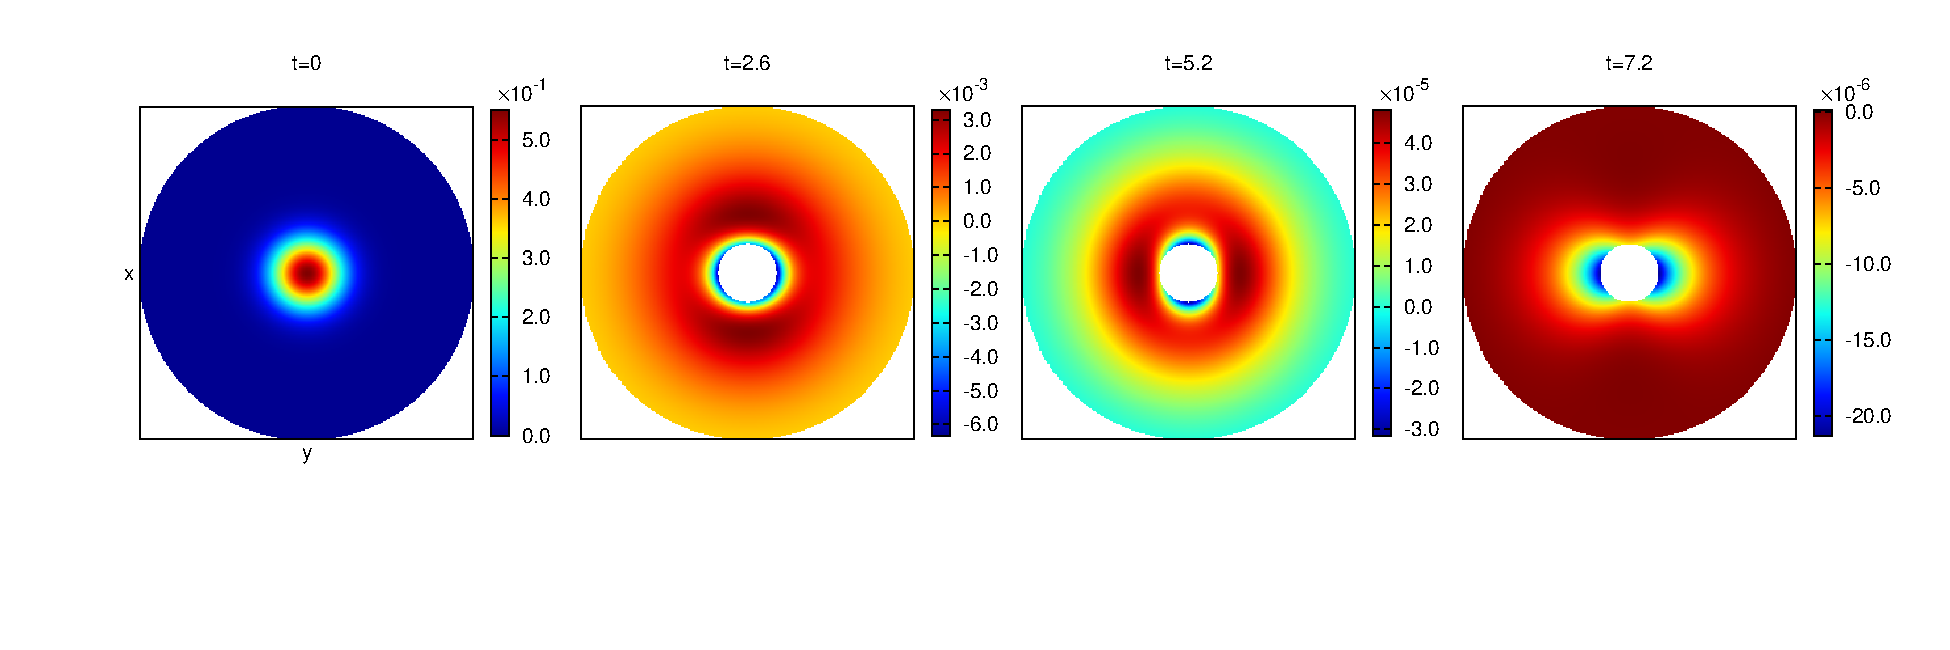
\includegraphics[width=7.0in,clip=true]{plots/bulkplots/L3/phi1/phi1_L3_snapshots_2.pdf}
\parbox{5.0in}{\caption{Snapshots of the scalar field on the $z=0$ slice.
        }\label{fig:snapshotsscalarfield-crop}}
\end{figure}

\begin{figure}[h]
        \centering
        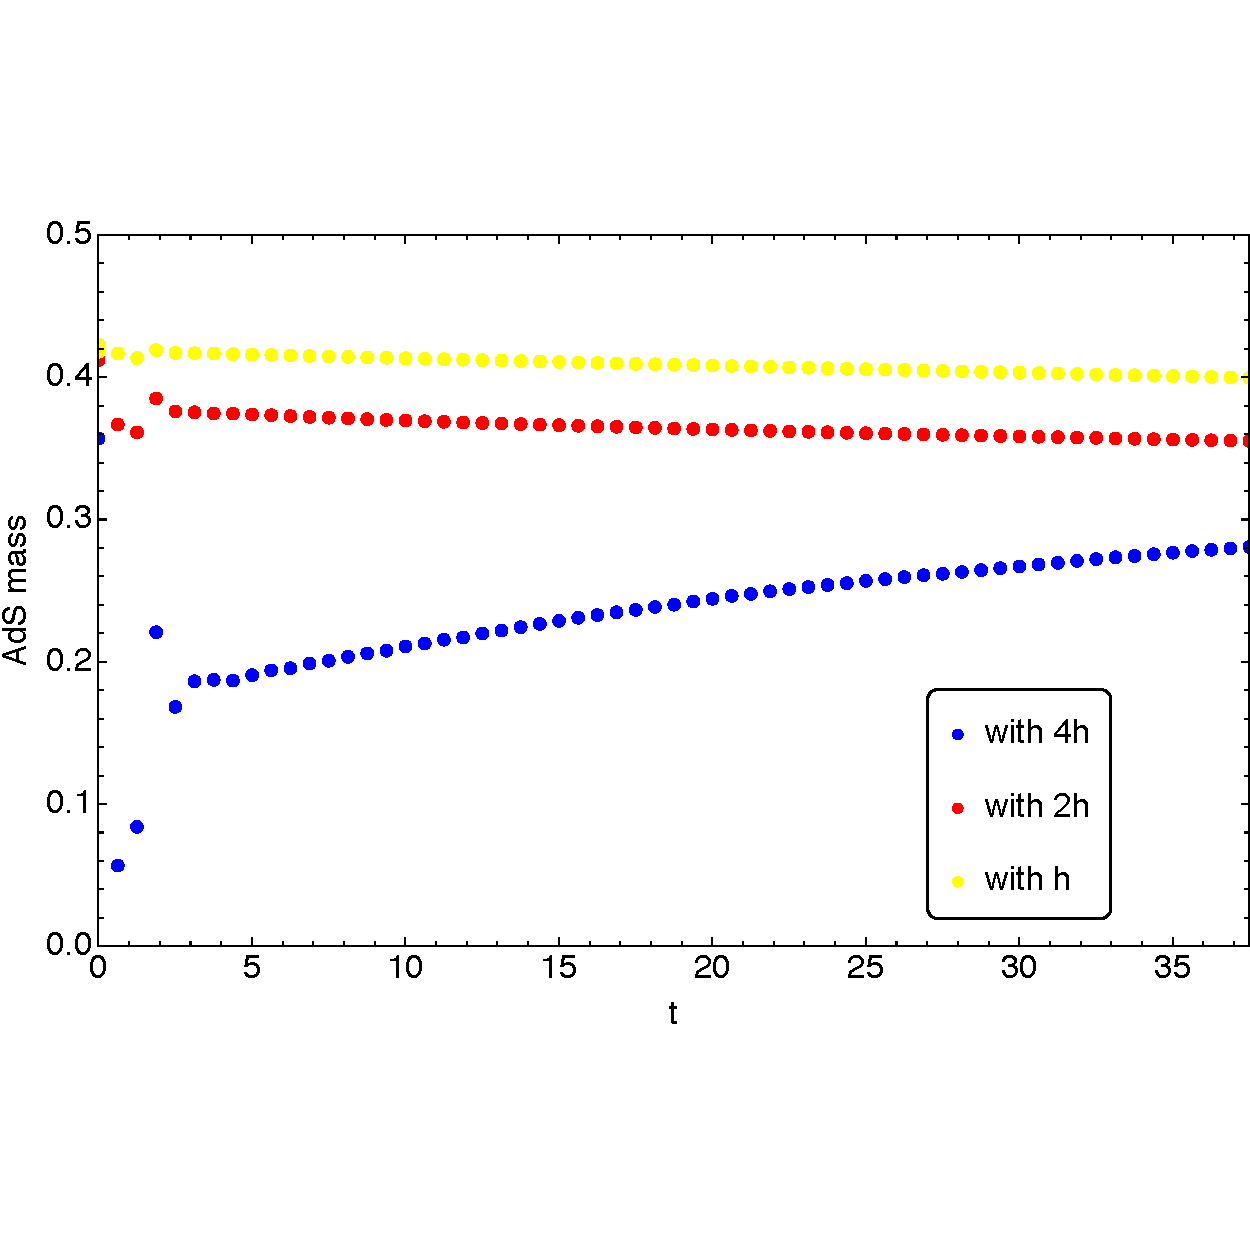
\includegraphics[width=4.0in,clip=true]{plots/timeseries/AdSmass/fullplotAdSmassL1L2L3res-cropped.pdf}
\parbox{5.0in}{\caption{Time series for AdS mass for different resolutions.
        }\label{fig:AdSmass-crop}}
\end{figure}

\begin{figure}[h]
        \centering
        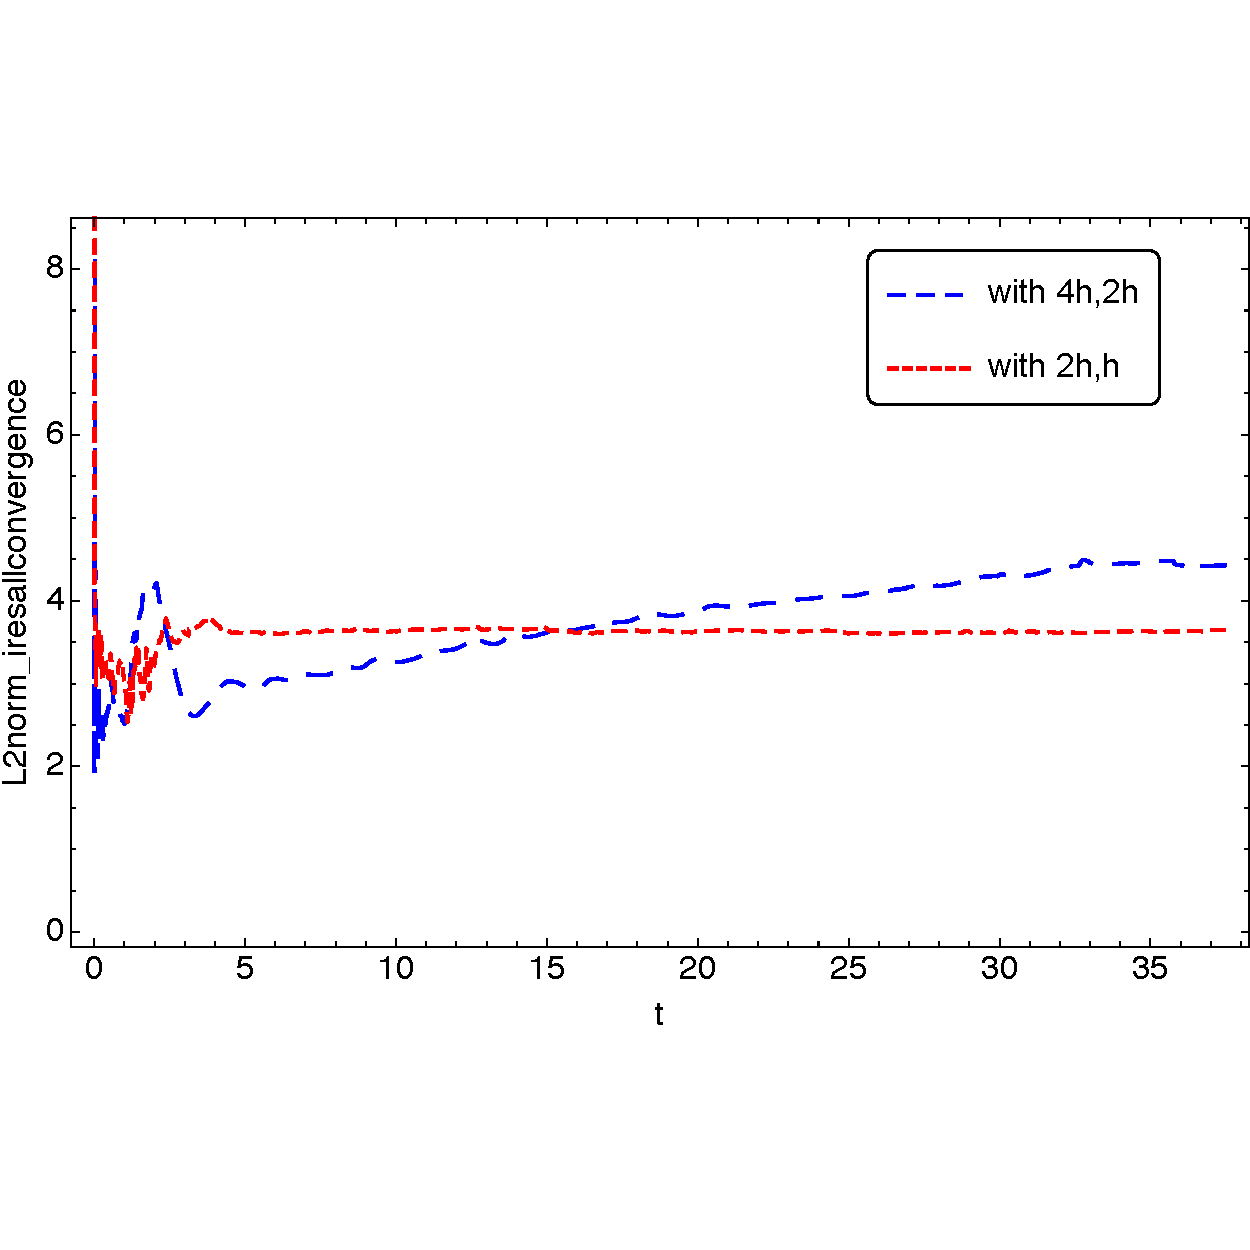
\includegraphics[width=4.0in,clip=true]{plots/timeseries/L2norm_iresallconvergence/fullplotiresallconvergenceL1L2L3res-cropped.pdf}
\parbox{5.0in}{\caption{Time evolution for $L^2$ norm of convergence factor for independent residual of EFE at different resolutions.
        }\label{fig:L2norm_iresallconvergence-crop}}
\end{figure}

\begin{figure}[h]
        \centering
        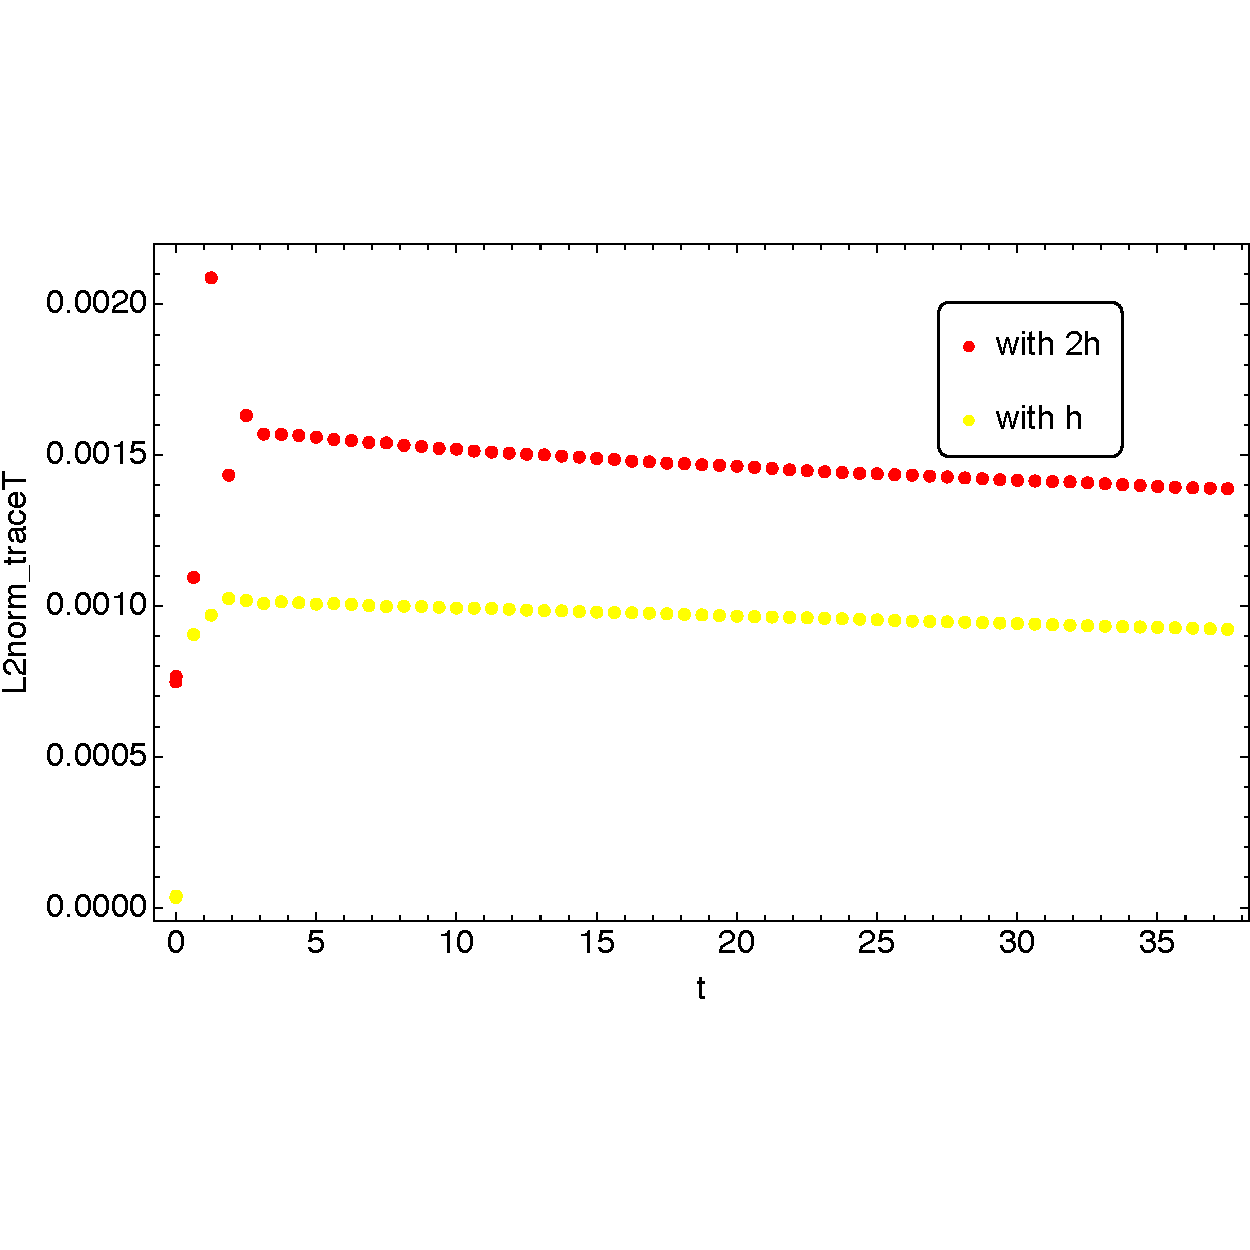
\includegraphics[width=4.0in,clip=true]{plots/timeseries/L2norm_quasiset_trace/fullplotL2normtraceL2L3res-cropped.pdf}
\parbox{5.0in}{\caption{Time evolution for $L^2$ norm of trace of quasi-local energy-momentum tensor of the boundary CFT at different resolutions.
        }\label{fig:L2norm_quasisettrace-crop}}
\end{figure}

\begin{figure}%
    \centering
    \subfloat[x-dependency]{{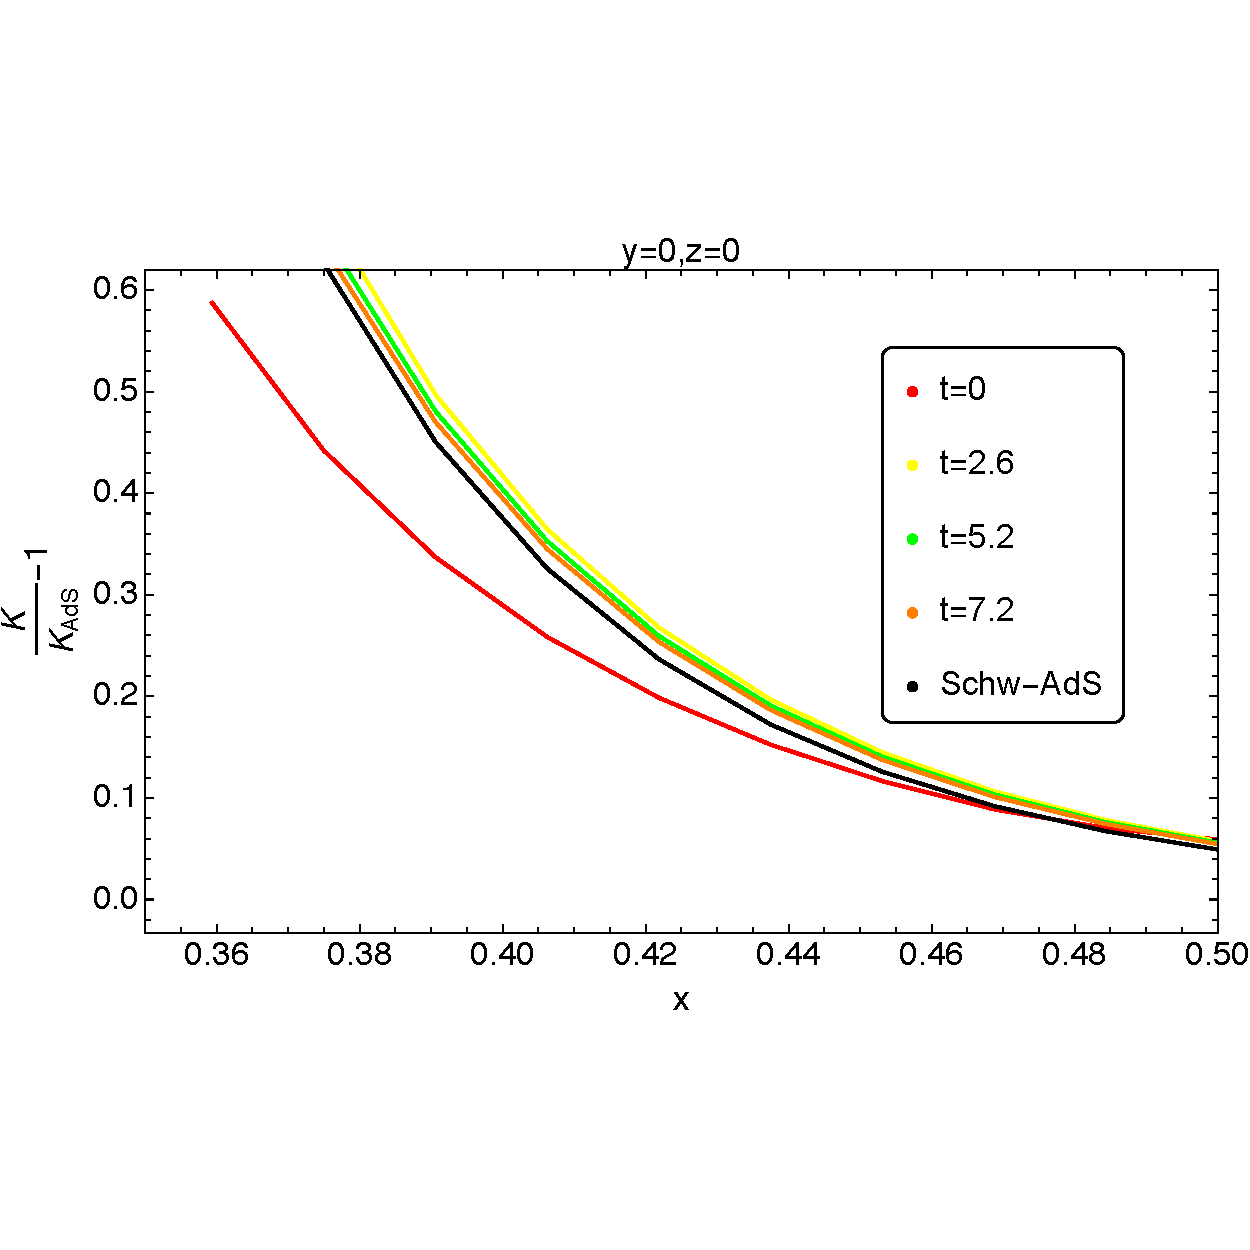
\includegraphics[width=3.0in]{plots/bulkplots/L2/relkretsch/fullplotxcoordrelkretschL2res-cropped.pdf} }}%
    \qquad
    \subfloat[y-dependency]{{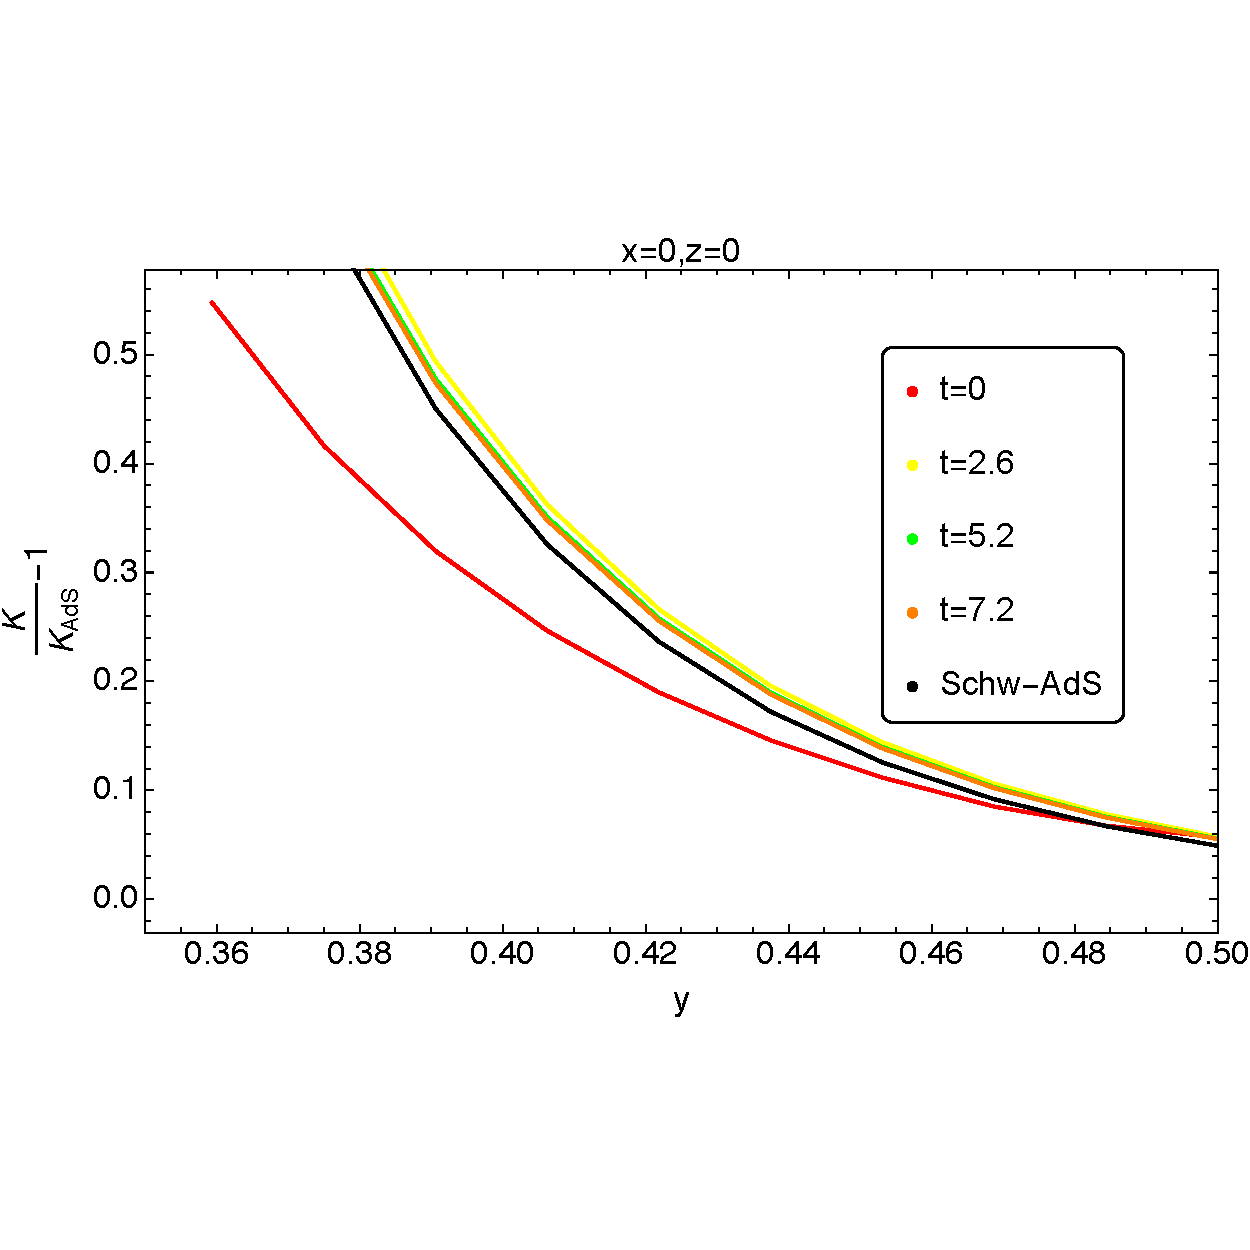
\includegraphics[width=3.0in]{plots/bulkplots/L2/relkretsch/fullplotycoordrelkretschL2res-cropped.pdf} }}%
    \caption{Time evolution of Kretschmann: the Kretschmann scalar of the solution approaches the one for Schwarzschild-AdS}%
    \label{fig:example}%
\end{figure}




\section{Discussion}\label{sec:Discussion}

\ack
Simulations were run on the {\bf Apocrita} cluster at Queen Mary University of London.

\appendix
\section{Generalized Harmonic Formulation}

The generalized harmonic formulation of the Einstein equations is based on coordinates $x^\mu$ that each satisfies a wave equation $\Box x^{\mu}=H^\mu$ with source functions $H^\mu$.
As long as the constraint $0=C^\mu \equiv H^\mu-\Box x^\mu$ is satisfied, we can then write the trace-reversed Einstein equations in $d$ dimensions with cosmological constant $\Lambda$
\begin{equation}
0=R_{\mu\nu} - \frac{2\Lambda}{d-2} g_{\mu\nu} - 8\pi\left( T_{\mu\nu} - \frac{1}{d-2} T g_{\mu\nu} \right)
\end{equation}
as
\begin{eqnarray}
0
&=& R_{\mu\nu} - \nabla_{(\mu} C_{\nu)} - \frac{2\Lambda}{d-2} g_{\mu\nu} - 8\pi\left( T_{\mu\nu} - \frac{1}{d-2} {T^\alpha}_\alpha g_{\mu\nu} \right) \nonumber \\
&=& R_{\mu\nu} - \nabla_{(\mu} H_{\nu)} + \nabla_{(\mu} \Box{x}_{\nu)} - \frac{2\Lambda}{d-2} g_{\mu\nu} - 8\pi\left( T_{\mu\nu} - \frac{1}{d-2} {T^\alpha}_\alpha g_{\mu\nu} \right) \nonumber \\
&=& -\frac{1}{2} g^{\alpha\beta} g_{\mu\nu,\alpha\beta} - g^{\alpha\beta}{}_{,(\mu}g_{\nu)\alpha,\beta} - H_{(\mu,\nu)} + H_\alpha \Gamma^\alpha{}_{\mu\nu} \nonumber \\
&&- \Gamma^\alpha{}_{\mu\beta}\Gamma^\beta{}_{\alpha\nu} - \frac{2\Lambda}{d-2} g_{\mu\nu} - 8\pi\left( T_{\mu\nu} - \frac{1}{d-2} {T^\alpha}_\alpha g_{\mu\nu} \right) \nonumber,
\end{eqnarray}
where the choice of $H_\mu = g_{\mu\nu} H^\nu$ constitutes a gauge choice. 
To suppress constraint-violating solutions that do not satisfy $C_\mu=0$, we supplement with constraint-damping terms as introduced in~\cite{Gundlach:2005eh} and obtain our final form of the Einstein equations
\begin{eqnarray}\label{eqn:efe_gh_modified}
&-& \frac{1}{2} g^{\alpha \beta} g_{\mu \nu, \alpha \beta} - 
{g^{\alpha \beta}}_{,(\mu} g_{\nu) \alpha, \beta} - H_{(\mu, \nu)} + H_\alpha {\Gamma^\alpha}_{\mu \nu} \nonumber \\
&-& {\Gamma^\alpha}_{\beta \mu} {\Gamma^\beta}_{\alpha \nu} - \kappa \left( 2 n_{(\mu} C_{\nu)} - (1+P) g_{\mu \nu} n^\alpha 
C_\alpha \right) \nonumber \\
&=&   \frac{2}{d-2} \Lambda g_{\mu \nu} + 8\pi \left( T_{\mu \nu} - 
\frac{1}{d-2} {T^\alpha}_\alpha g_{\mu \nu} \right).
\end{eqnarray}

\section{Convergence Tests in the Bulk}\label{sec:convbulk}

Here we display a pair of numerical tests that demonstrate convergence trends for a representative simulation with no mesh refinement.
We do this for [pick simulation] with initial data parameters [display parameters]

Let us denote the value of the field $f$ at the point $(t,x,y,z)$ in a simulation with mesh spacing $\Delta$ by $f_\Delta(t,x,y,z)$.
To show that the solution $f_\Delta(t,x,y,z)$ converges to a function $f(t,x,y,z)$ in the continuum limit $\Delta\rightarrow0$, we compute the rate of convergence $Q(t,x,y,z)$ at each point of interest
\begin{equation}\label{eq:qconv}
Q(t,x,y,z)=\frac{1}{\ln(3/2)}\ln\left( \frac{f_{9h/4}(t,x,y,z)-f_{3h/2}(t,x,y,z)}{f_{3h/2}(t,x,y,z)-f_{h}(t,x,y,z)} \right).
\end{equation}
We use second-order accurate finite difference stencils, and there is a factor of 3/2 between successive resolutions.
Thus, we expect $Q$ to asymptote to $Q=2$ in the limit $\Delta\rightarrow0$.

To show that the solution is converging to a solution of the Einstein equations, we compute an independent residual. 
This is obtained by taking the numerical solution and substituting it into a discretized version of
the Einstein equations, a component of which we denote $\Phi_\Delta$. 
The independent residual should be purely numerical truncation error, so we can compute a convergence factor for it by using only two resolutions
\begin{equation}\label{eq:qires}
Q_{EFE}(t,x,y,z)=\frac{1}{\ln(3/2)}\ln\left( \frac{\Phi_{3h/2}(t,x,y,z)}{\Phi_{h}(t,x,y,z)} \right).
\end{equation}
Again, with second-order accurate finite difference stencils and with a factor of 3/2 between successive resolutions, we expect $Q$ to approach $Q=2$ as $\Delta\rightarrow0$.

\section{Extrapolation Technique and Convergence at AdS Boundary}\label{sec:extrapconvbdy}

As explained in Section~\ref{sec:results}, given a Cartesian grid with spacing $\Delta$, since the AdS boundary generally does not lie on points of the grid, we can only obtain the approximated value $f^{bdy}_{\Delta}$ of any boundary quantity $f$ through extrapolation, using the numerical values of $f$ on grid points near the boundary, which we denote by $f_\Delta$. In this Section  we describe how grid points are chosen for extrapolation and we show convergence by computing the factor \eref{eq:qconv} for $f^{bdy}_{\Delta}$ at boundary points.

If we wish to test convergence of $f^{bdy}_{\Delta}$ in the continuum limit $\Delta\rightarrow0$, there are two crucial criteria for the choice of grid points that are \emph{suitable} for extrapolation. We will now explain them with the help of Fig.~\ref{fig:lego_circle}, which shows an example of the result of the application of these criteria in the first quadrant of a $z=const.$ surface of the grid for first order extrapolation.
\begin{enumerate}
 \item Consider the value of $f^{bdy}_{\Delta}$ at any boundary point $p_{bdy}$. If we obtain this by $n^{th}-$order extrapolation, $f^{bdy}_{\Delta}(p_{bdy})$ is a combination of the values $f_\Delta(p_1),f_\Delta(p_2),\dots,f_\Delta(p_{n+1})$ (where $p_1,p_2,\dots,p_{n+1}$ are the bulk points used for extrapolation) multiplied by factors that depend on the coordinates of $p_{bdy},p_1,\dots,p_{n_{\Delta}+1}$. Therefore, we can write  $f^{bdy}_{\Delta}(p_{bdy})=f(p_{bdy})+c_{extr}(p_{bdy},p_1,p_2,\dots,p_{n+1})+c_\Delta(p_1,p_2,\dots,p_{n+1})\Delta^2$ where the first term is the true value of $f$ at $p_{bdy}$, the second term is the error due to the extrapolation approximation and the third term is the error coming from the numerical error in $f_\Delta$. From this we immediately see that the convergence factor \eref{eq:qconv} at point $p_{bdy}$ can be expected to asymptote to 2 as $\Delta\rightarrow0$ only if the points $p_1,p_2,\dots,p_{n+1}$ are the same for all 3 resolutions involved.
 
 \item For each resolution, grid points with $\rho\geq 1-\Delta/2$ (i.e. points outside the dotted line in Fig.~\ref{fig:lego_circle}) are excised due to the fact that some quantities diverge at $\rho=1$, the value of functions at points with $1-3\Delta/2\leq \rho < 1-\Delta/2$ (i.e. points between the dotted line and the dashed line in Fig.~\ref{fig:lego_circle}) are set by using forward/backward stencils, and the value of functions at points with $1-5\Delta/2\leq \rho < 1-3\Delta/2$ (i.e. points between the dashed line and the continuous blue line in Fig.~\ref{fig:lego_circle}) are set by using centred stencils which, however, use neighbouring points set by forward/backward stencils. For all these reasons, we can only expect convergence if we pick grid points with  $\rho<1-5\Delta/2$.
 \end{enumerate}
Furthermore, among the points satisfying (i) and (ii), we want the ones that are closest to the boundary in order for extrapolation to provide a more accurate approximation.

\begin{figure}[h]
        \centering
        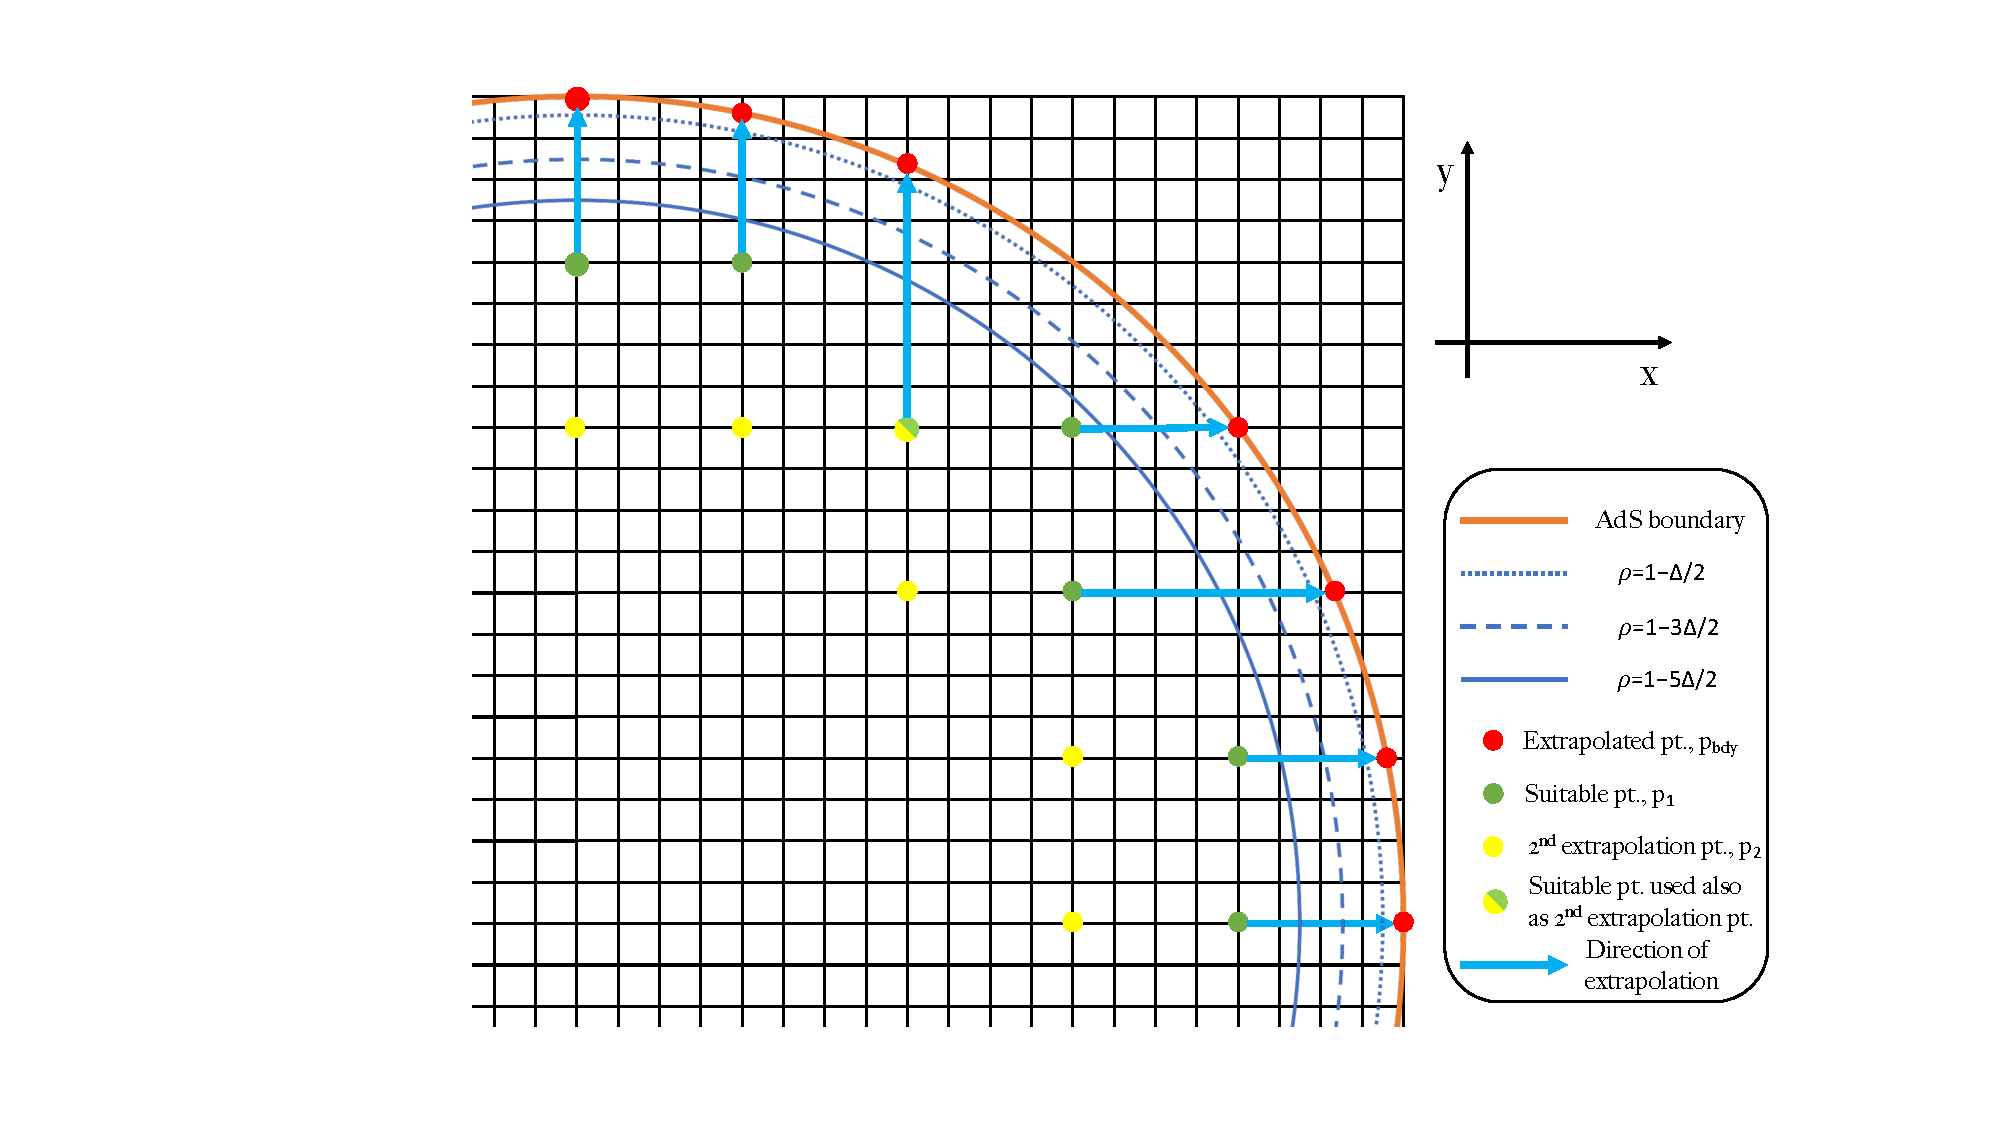
\includegraphics[width=6.0in,clip=true]{plots/lego_circle/Lego_circle.pdf}
\parbox{5.0in}{\caption{Visual description of first order extrapolation technique in the first quadrant of a $z=const.$ surface for the lowest resolution, with grid spacing $\Delta$, among the 3 involved in a convergence test ($const.$ is chosen as the $z-$coordinate value of one of the points common to all 3 resolutions). We show a typical example in which common points are 4 grid points away from each other along each direction.
        }\label{fig:lego_circle}}
\end{figure}
 
Once suitable points have been found (the green dots in Fig.~\ref{fig:lego_circle}), the extrapolation technique proceeds as follows:
 \begin{itemize}
 \item consider the first suitable point, $p_1$, and identify the coordinate with the largest value, e.g. $x$, and its sign, e.g. $x>0$.
 \item take the next $n$ points, $p_2,\dots,p_{n+1}$, used for $n^{th}-$order extrapolation along the identified axis ($x$ in our example) in the direction of the bulk (decreasing $x$ in the example), making sure that they also satisfy (i) ((ii) is trivially satisfied by construction). For the case of first order extrapolation, each $p_2$ is represented in yellow in Fig.~\ref{fig:lego_circle}.
 \item use $n^{th}-$ order extrapolation on $f_\Delta(p_1),\dots,f_\Delta(p_{n+1})$ to determine the value of $f^{bdy}_{\Delta}(p_{bdy})$ where $p_{bdy}$ is the boundary point along the identified axis in the direction of the boundary (one of the red dots in Fig. ~\ref{fig:lego_circle}). In our example, $p_{bdy}$ is the point with coordinates $(x,y,z)=(\sqrt{1-y(p_1)^2-z(p_1)^2},y(p_1),z(p_1))$.
 \item repeat the previous steps until the last suitable point.
 \end{itemize}

CONVERGENCE PLOTS

Notice that the convergence test \eref{eq:qires} cannot be performed at the boundary for functions with true value 0 (such as $<trT>_{CFT}$), because their extrapolated value is not just the term linear in $\Delta^2$ but it also includes the extrapolation error $c_{extr}$.



%-------------------------------------------------------
% Bibliography
%-------------------------------------------------------
\section*{References}
\bibliographystyle{iopart-num}
\bibliography{3p1}



\end{document}

